\documentclass[]{article}
\usepackage{lmodern}
\usepackage{amssymb,amsmath}
\usepackage{ifxetex,ifluatex}
\usepackage{fixltx2e} % provides \textsubscript
\ifnum 0\ifxetex 1\fi\ifluatex 1\fi=0 % if pdftex
  \usepackage[T1]{fontenc}
  \usepackage[utf8]{inputenc}
\else % if luatex or xelatex
  \ifxetex
    \usepackage{mathspec}
  \else
    \usepackage{fontspec}
  \fi
  \defaultfontfeatures{Ligatures=TeX,Scale=MatchLowercase}
\fi
% use upquote if available, for straight quotes in verbatim environments
\IfFileExists{upquote.sty}{\usepackage{upquote}}{}
% use microtype if available
\IfFileExists{microtype.sty}{%
\usepackage[]{microtype}
\UseMicrotypeSet[protrusion]{basicmath} % disable protrusion for tt fonts
}{}
\PassOptionsToPackage{hyphens}{url} % url is loaded by hyperref
\usepackage[unicode=true]{hyperref}
\hypersetup{
            pdfborder={0 0 0},
            breaklinks=true}
\urlstyle{same}  % don't use monospace font for urls
\usepackage{graphicx,grffile}
\makeatletter
\def\maxwidth{\ifdim\Gin@nat@width>\linewidth\linewidth\else\Gin@nat@width\fi}
\def\maxheight{\ifdim\Gin@nat@height>\textheight\textheight\else\Gin@nat@height\fi}
\makeatother
% Scale images if necessary, so that they will not overflow the page
% margins by default, and it is still possible to overwrite the defaults
% using explicit options in \includegraphics[width, height, ...]{}
\setkeys{Gin}{width=\maxwidth,height=\maxheight,keepaspectratio}
\IfFileExists{parskip.sty}{%
\usepackage{parskip}
}{% else
\setlength{\parindent}{0pt}
\setlength{\parskip}{6pt plus 2pt minus 1pt}
}
\setlength{\emergencystretch}{3em}  % prevent overfull lines
\providecommand{\tightlist}{%
  \setlength{\itemsep}{0pt}\setlength{\parskip}{0pt}}
\setcounter{secnumdepth}{0}
% Redefines (sub)paragraphs to behave more like sections
\ifx\paragraph\undefined\else
\let\oldparagraph\paragraph
\renewcommand{\paragraph}[1]{\oldparagraph{#1}\mbox{}}
\fi
\ifx\subparagraph\undefined\else
\let\oldsubparagraph\subparagraph
\renewcommand{\subparagraph}[1]{\oldsubparagraph{#1}\mbox{}}
\fi

% set default figure placement to htbp
\makeatletter
\def\fps@figure{htbp}
\makeatother


\date{}

\begin{document}

\section{Towards Proving Application Isolation for Cryptocurrency
Hardware
Wallets}\label{towards-proving-application-isolation-for-cryptocurrency-hardware-wallets}

Andrew Shen

\subsection{1 Introduction}\label{introduction}

Modern personal computers (PCs) often contain numerous security
vulnerabilities due to bugs in their complex operating systems, which
have millions of lines of code{[}1{]}. In other words, the size of the
Trusted Computing Base (TCB), or the code assumed to be implemented
correctly, is relatively large, and as a result, writing a bug-free
operating system on the scale of Linux or Windows is nearly impossible.
However, many applications that might run on the PC including
cryptocurrency or banking software require strong guarantees to ensure
secure transactions. The security guarantees provided by PCs are
insufficient for these security sensitive operations. Hardware wallets,
small devices with an independent operating system, provide the
capabilities to isolate these sensitive operations and complete them
securely. Hardware wallets have a screen and buttons used to authorize
and sign transactions and connect to the PC through a USB port. This
allows for the application to be split into two parts where the majority
of the application still runs on the PC, but the secure transaction
approval step occurs on the hardware wallet. Figure 1.1 illustrates this
process. The private keys used to sign the transactions are stored
solely on the hardware wallet, completely isolating them from the PC.
Because hardware wallets only need to perform a small subset of the
operations that a PC would, they use a significantly smaller operating
system. With a smaller codebase and TCB, there would be less room for
attacks and fewer bugs. Rather than trusting the PC, the user only needs
to trust that the hardware wallet works as intended. For example, a
compromised PC would be unable to steal Bitcoin from a hardware wallet
as it would be unable to access the confidential information stored
solely on the hardware wallet. If the PC tried to perform a malicious
action, the hardware wallet would receive the transaction and then
display the exact transaction it received on the screen. This way if the
compromised PC requested a malicious transaction, for example, the user
could decline said transaction. There is no other method of signing the
transaction other than using the private keys, which reside solely on
the hardware wallet.

\begin{figure}
\centering
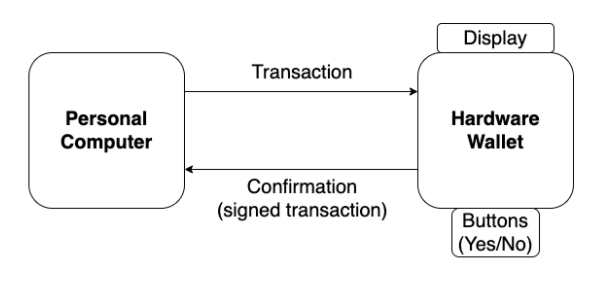
\includegraphics{Hardware-Wallet-Diagram.png}
\caption{}
\end{figure}

\textbf{Figure 1.1.} A diagram of a hardware wallet receiving and
approving a transaction from the PC after the user has physically
confirmed the transaction shown on the display using the buttons on the
hardware wallet.

Although operating systems on hardware wallets are less complex than
those on PCs, they are still prone to error and have many thousands of
lines of code{[}2{]}. For example, security vulnerabilities have been
previously discovered in modern hardware wallets such as Ledger. These
vulnerabilities range from hardware misconfiguration bugs that can be
abused without even leaving user mode to system call argument validation
bugs in the kernel. One method used to eliminate these sorts of bugs is
by using formal verification, a technique used to reason about the
behavior of a program. Prior work such as HV6{[}3{]} and Serval{[}4{]}
tackle verifying a desktop-style operating system by using push-button
formal verification. However, these previous works only reason about
individual system calls and do not reason about code that runs between
these system calls in user mode. One bug that Serval would not detect
would be a misconfigured physical memory protection (PMP) register,
which would allow user code to access memory that it should not. We seek
to reduce the TCB further by using formal verification to eliminate
certain classes of bugs that could be exploited while running in user
mode. One such security property would be guaranteeing that user code is
unable to modify any memory that it is not permitted to access. To
accomplish this task, we build a kernel in RISC-V, which represents a
simplified version of an actual hardware wallet kernel. In addition, we
also build a QEMU-like symbolic machine emulator to reason about the
behavior of our kernel. This machine emulator differs from QEMU in that
it can reason about symbolic values in the machine state, essentially
allowing us to reason about machine execution even when some aspects
such as the user code are unknown, which allows us to reason about
arbitrary user mode code. This enables us to state and prove important
security properties such as the inability of code running in user mode
to change RAM of protected regions. We prove that applications cannot
tamper with the isolation set up while executing in user mode. With
proofs further reasoning about system calls, we could complete an
end-to-end proof about the system's execution. Although this is not yet
an end-to-end correctness proof, we prove important properties that are
also useful.

\subsection{2 Approach}\label{approach}

\subsubsection{2.1 Kernel Design}\label{kernel-design}

We built a kernel similar to one found in a real hardware wallet. We
design our kernel to have the following features: the ability to
download, load, and run different applications. Also, we use a smaller
codebase to make debugging and reasoning easier. Our target hardware,
like other hardware wallets, has no virtual memory support. To isolate
the kernel from the user application we use RISC-V M-mode as our
privileged level with unrestricted access to memory and use RISC-V
U-mode for running user applications, which has only restricted access
to memory due to our PMP register setup. The kernel begins with turning
on and booting the kernel, where several control register configurations
occur to set up proper privilege level settings. These boot-time
operations include configuring the PMP registers in such a way that user
applications can only access a predefined region of memory they are
permitted to use and giving the user the choice to download an
application or load an existing application to be run. Then, the kernel
executes the application that was selected by the user during boot time.
After finishing the execution of this program, the kernel stops, and to
run another application, the user must restart the kernel by physically
powering off and on the device; the kernel can only run a single
application within a single run. This simplifies the design of our
kernel making it easier to reason about while maintaining the same
functionality. Furthermore, our kernel does not need to support the same
multiplexing functionality that desktop PCs have as we only ever need to
run one cryptocurrency application at one time. \#\#\# 2.2 Verification
Our goal is to prove that our applications are isolated from one
another. To prove this property about our kernel, we must show that we
can set up our kernel in such a way that by the time we enter use mode,
the application is running in user mode and cannot modify confidential
memory. We use the PMP registers to restrict the user application memory
access as well as configure other critical registers at boot time
(mtvec, mstatus, etc) at boot time to create this state, which we will
refer to this configuration of kernel registers as being ``OK'' (Figure
2.1).

\begin{verbatim}
mtvec = 0x0000000080000080
pmpcfg0 = 0x000000000000001f
pmpcfg2 = 0x0000000000000018
pmpaddr0 = 0x000000002000bfff
pmpaddr1 = 0x0
pmpaddr1 = 0x0
pmpaddr2 = 0x0
pmpaddr3 = 0x0
pmpaddr4 = 0x0
pmpaddr5 = 0x0
pmpaddr6 = 0x0
pmpaddr7 = 0x0
pmpaddr8 = 0x7fffffffffffffff
pmpaddr9 = 0x0
pmpaddr10 = 0x0
pmpaddr11 = 0x0
pmpaddr12 = 0x0
pmpaddr13 = 0x0
pmpaddr14 = 0x0
pmpaddr15 = 0x0
\end{verbatim}

\textbf{Figure 2.1.} We define a state to be ``OK'' if the state has
specific registers configured as shown above.

Also, we must show that after booting up into this ``OK'' state and
switching to user mode for execution of the application, that any
instruction running in user mode causes exactly one of the following two
cases to occur: either the kernel remains in user mode and the kernel
maintains the ``OK'' property, or the kernel switches to kernel mode and
begins executing at the location predefined by the mtvec register, which
handles system calls (Figure 2.2). This corresponds to a standard
inductive proof where the base case is setting up our kernel into the
``OK'' state and the inductive step proves that no individual
instruction can tamper with protected RAM.

\begin{figure}
\centering
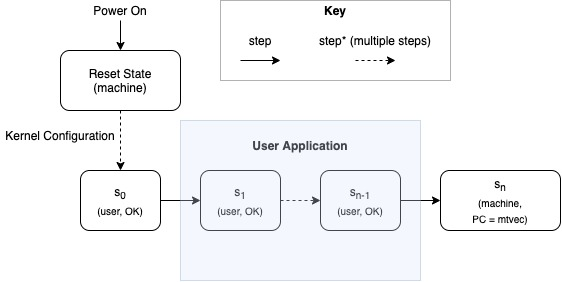
\includegraphics{Proof-Diagram.jpg}
\caption{}
\end{figure}

\textbf{Figure 2.2.} A diagram of the workflow of our kernel. The kernel
configures during the boot sequence until it reaches state s0, where s0
is the state of the machine immediately after the kernel boots up. Then
the kernel runs for an arbitrary number of steps n, where it remains in
U-mode and ``OK'' until it reaches state sn at which point it switches
to M-mode and begins executing at the address defined by mtvec.

Though we do not reason about system calls in our work, the system call
handler could be verified similarly to Serval and allows our user
application to perform different operations such as gaining access to
the UART, which handles input and output. Since any application is the
composition of many instructions, our proof covers all possible user
applications that could be run on the kernel including those with
illegal instructions. To complete the proof of these properties, we need
to employ symbolic values, which will allow us to reason about unknown
values in our machine. For the base case, only some registers and
regions of memory are defined, which allows us to use symbolic values to
represent the rest of the undefined parts of the machine. In the
inductive step, we use symbolic values to represent key parts of the
machine including the program counter and the user application region of
memory. This symbolic memory allows us to read an arbitrary instruction
from an arbitrary address and execute one instruction from our current
state s generating a new state s'. Using these two states, we can assert
that the confidential memory remains unchanged despite running this
arbitrary instruction on the address. If our assertion holds and there
exist no values for which the symbolic variables could be such that the
memory is changed between s and s', then this implies that it is not
possible under any circumstance that the memory was changed.
Furthermore, we can extend this to reason about the privilege level. We
can assert that either the mode is unchanged and remains in user mode or
exits user mode and begins executing at the address predetermined by the
mtvec register. This proof can be written as a more formal mathematical
formula as shown in Figure 2.3.

Base Case:

\begin{verbatim}
OK(s0), where s0 is the machine state immediately after the boot sequence.
\end{verbatim}

Induction Case:

\begin{verbatim}
∀s, s′ : OK(s) ⟹ s′ = step(s) ⟹ is_user(s′) ∧ OK(s) ⟹ 
(is_user(s′) ∧ OK(s′)) ∨ (is_m(s′) ∧ pc(s′) = mtvec(s))
\end{verbatim}

\textbf{Figure 2.3.} The proof expressed in more formal terms using
mathematical notation.

\subsubsection{2.3 Symbolic RISC-V Machine
Emulator}\label{symbolic-risc-v-machine-emulator}

To implement a machine emulator that works with symbolic variables, we
turn to the Rosette language, an extension of the Racket language, which
allows us to lift regular Racket code to be able to operate with
symbolic values. We can write the kernel emulator in Racket and use
Rosette to lift that emulator to function as a symbolic emulator capable
of operating on arbitrary instructions. Mirroring the implementation of
a regular machine emulator, the workflow of the emulator, we separate
the execution of each instruction into three functions: fetch, decode
(Figures 2.4 and 2.5), execute (Figure 2.6). The fetch functions
extracts the raw bits that make up the instruction from RAM. The next
function, decode, decodes those raw bits and based on the RISC-V
specification, interprets which instruction and parameters to run. The
final function, execute, emulates the decoded instruction and executes
it on our machine state updating all necessary values such as the
program counter. These functions are combined in the step function
(Figure 2.7) to make up what we refer to as applying one ``step'' on our
state in Figures 2.1 and 2.2.

\begin{verbatim}
(define (decode m b_instr)
    (define instr null)
    (define opcode (extract 6 0 b_instr))
    (define fmt (get-fmt m opcode))
    (cond
        [(eq? fmt 'R)
        (decode-R m b_instr)]
    [(eq? fmt 'I)
        (decode-I m b_instr)]
    [...]
    [else
        (illegal-instr m)]))
(provide decode)
\end{verbatim}

\textbf{Figure 2.4.} A snippet of the \texttt{decode} function used to
retrieve the instruction and parameters from a byte string.

\begin{verbatim}
(define (decode-R m b_instr)
    (define op null)
    (define rd (extract 11 7 b_instr))
    (define funct3 (extract 14 12 b_instr))
    [...]
    (define valid null)
    (cond
        [(and (bveq funct3 (bv #b000 3))
                (bveq funct7 (bv #b0000000 7)))
                (list 'add rd rs1 rs2)]
        [(and (bveq funct3 (bv #b000 3))
                (bveq funct7 (bv #b0100000 7)))
                (list 'sub rd rs1 rs2)]
        [...]
        [else
            (illegal-instr m)]))
\end{verbatim}

\textbf{Figure 2.5.} A snippet of a utility function used by the main
\texttt{decode} function to decode ``R-Format'' instructions, one of the
few types of formats possible.

\begin{verbatim}
(define (execute instr m)
    (define opcode (list-ref instr 0))
    (define pc (get-pc m))
    (cond
        [(eq? opcode 'lb)
            (define rd (list-ref-nat instr 1))
            (define v_rs1 (gprs-get-x m (list-ref-nat instr 2)))
            [...]
            (define val (sign-extend (machine-ram-read m adj_addr 1)
                                    (bitvector 64)))
            (gprs-set-x! m rd val)
            (set-pc! m (bvadd pc (bv 4 64)))
            instr]
        [(eq? opcode 'sb)
            (define v_rs1 (gprs-get-x m (list-ref-nat instr 1)))
            [...]           
            (define success (machine-ram-write! m adj_addr v_rs2 8))
            instr])]))
\end{verbatim}

\textbf{Figure 2.6.} A snippet of the \texttt{execute} function, which
takes a decoded instruction and executes it, applying the result on the
state of the machine \texttt{m}.

\begin{verbatim}
(define (step m)
    (define next_instr (get-next-instr m)) ; fetch raw instruction
    (define decoded_instr (decode m next_instr))
    (execute decoded_instr m))
\end{verbatim}

\textbf{Figure 2.7.} The \texttt{step} function is analogous to the
\texttt{step} referenced by the proof. Each step fetches, decodes, and
executes one instruction from the machine \texttt{m} RAM.

\subsubsection{2.4 Challenges}\label{challenges}

Oftentimes, due to the nature of Rosette, it can be beneficial to
express certain values or data in different ways, which are easier for
Rosette to generate simpler terms. One such example of this is the
memory, which the symbolic machine emulator maintains. At first glance,
it might seem intuitive to use an array representation for the memory,
which is actually quite good for quick memory reads and writes when
simulating actual code with concrete values. The major pitfall with this
implementation becomes apparent when proving the unchanged confidential
memory aspect of our proof. To completely verify that the entire region
of confidential memory is unchanged, it is necessary to prove that each
individual address remains unchanged. This results in the time to run
our proof growing linearly with the size of the array and subsequently,
the size of the RAM. Figure 2.9 demonstrates the issue with writes to
memory using symbolic addresses. When we try to run the proof with 128
megabytes of RAM, we find that it takes an unreasonable amount of time
to complete the proof and therefore, turn to an alternative
implementation. We instead decide to use an uninterpreted function
representation of memory where memory is represented as a function that
takes an address and returns the value at that address. Then each time
we wish to write a value v to an address a, we essentially wrap our
current memory function in an if case that returns the value v if the
user tries to get address a and the old memory function applied to the
address if the address is not a. The Racket implementation of these two
memory representations is described in Figure 2.8. Furthermore, the
benefits of using uninterpreted function based memory is illustrated in
the constant size term produced even after writing to an address as
shown in Figure 2.9.

\begin{verbatim}
(define (uf-memory-write! mem addr val)
  (lambda (addr*)
    (if (bveq addr addr*)
      val
      (mem addr*))))

(define (uf-memory-read mem addr)
  (mem addr))

(define (array-memory-write! mem addr val)
  (vector-set! mem addr val))

(define (array-memory-read mem addr)
  (vector-ref mem addr))
\end{verbatim}

\textbf{Figure 2.8.} Rosette implementation of read and write for
array-based memory and uninterpreted function (uf) based memory.

\begin{verbatim}
(define array_memory (vector 0 1 2))
(define-symbolic* idx integer?)
(define-symbolic* pos val integer?)

(printf "Before Write: ~a~n" (array-memory-read array_memory idx))
(array-memory-write! array_memory pos val)
(printf "After Write: ~a~n" (array-memory-read array_memory idx))

; >>> Before Write: (ite* (⊢ (= 0 idx$0) 0) (⊢ (= 1 idx$0) 1) (⊢ (= 2 idx$0) 2))
; >>> After Write: (ite* (⊢ (= 0 idx$0) (ite (= 0 pos$0) val$0 0)) (⊢ (= 1 idx$0)
                    (ite (= 1 pos$0) val$0 1)) (⊢ (= 2 idx$0) (ite (= 2 pos$0) val$0 2)))

(define uf_memory (fresh-symbolic fnmem (~> integer? integer?)))
(uf-memory-write! uf_memory 0 0)
(uf-memory-write! uf_memory 1 1)
(uf-memory-write! uf_memory 2 2)

(printf "Before Write: ~a~n" (uf-memory-read uf_memory idx))
(uf-memory-write! uf_memory pos val)
(printf "After Write: ~a~n" (uf-memory-read uf_memory idx))

; >>> Before Write: (app fnmem$0 idx$0)
; >>> After Write: (app fnmem$0 idx$0)
\end{verbatim}

\textbf{Figure 2.9.} An example demonstrating how terms generated from
reading and writing to array based memory are much larger and complex
than those generated from uninterpreted function based memory. In this
example, both memory representations begin with the values 0, 1, and 2
in the index 0, 1, and 2 respectively, then write the symbolic integer
\texttt{val} to position \texttt{pos} in the memory representation. The
print statements corresponding to \texttt{Before\ Write:} and
\texttt{After\ Write:} refer to the terms generated by reading from a
symbolic index. The array based memory term grows significantly, while
the uninterpreted function based memory term remains constant.

\subsection{3 Evaluation}\label{evaluation}

We evaluate our work on two factors: whether or not the verification
terminated in a reasonable amount of time and which bugs were eliminated
by our proof. For reasonable machine settings, notably 1 MB of RAM, both
the base case and the recursive of the proof finish execution in roughly
25 minutes and 5 seconds respectively. With respect to the bugs
eliminated, we cover a few major cases. Most prominently, bugs that
occur with misconfigurations in the kernel boot sequence. These include
incorrectly configured PMP registers and incorrect privilege level set
up when entering user application execution, both of these bugs would
allow user mode applications to access confidential memory it should not
have access.

\subsubsection{3.1 Limitations}\label{limitations}

Though our symbolic machine emulator implements enough of the RISC-V
instruction set to boot our simple kernel, we have only implemented 42
of the 100+ instructions in the extended specification. With this added
functionality, we would be able to complete the end-to-end proof by
using verification techniques similar to those in Serval on these system
calls. Finally, the emulation of the boot sequence runs somewhat slowly
for large sizes of RAM, which we would like to investigate further and
hope to improve.

\subsection{4 Related Work}\label{related-work}

HV6 and Serval use push-button verification to prove properties about
system calls operating in kernel mode for desktop-like operating
systems. sel4{[}5{]} uses a manual proof with Isabelle, a proof
assistant, to prove the correctness of a microcontroller style kernel
for use on an embedded device. CertiKOS{[}6{]} is another recent work
that also uses proof assistants to prove security properties about their
kernel, which has the unique capability of supporting concurrent
operations. This technique uses a high level of effort to construct the
proof.

\subsection{5 Conclusion}\label{conclusion}

We make progress on developing a proof of end-to-end correctness for
application isolation on cryptocurrency hardware wallets by using formal
verification techniques. We build a kernel and symbolic machine
emulator, which can reason about the machine state even when some
aspects are unknown, and prove that we can set up the kernel at boot
time in such a way that user applications are properly isolated and are
unable to modify private memory.

\subsection{References}\label{references}

\begin{enumerate}
\def\labelenumi{\arabic{enumi}.}
\tightlist
\item
  https://ostoday.org/windows/how-many-lines-of-code-in-windows-10.html
\item
  https://www.riscure.com/uploads/2018/08/Riscure\_Hacking\_Secure\_Cryptowallet.pdf
\item
  https://unsat.cs.washington.edu/papers/nelson-hyperkernel.pdf
\item
  https://unsat.cs.washington.edu/papers/nelson-serval.pdf
\item
  https://www.sigops.org/s/conferences/sosp/2009/papers/klein-sosp09.pdf
\item
  https://www.usenix.org/system/files/conference/osdi16/osdi16-gu.pdf
\end{enumerate}

\end{document}
